\documentclass[a4paper, 14pt]{extarticle}

% Поля
%--------------------------------------
\usepackage{geometry}
\geometry{a4paper,tmargin=2cm,bmargin=2cm,lmargin=3cm,rmargin=1cm}
%--------------------------------------


%Russian-specific packages
%--------------------------------------
\usepackage[T2A]{fontenc}
\usepackage[utf8]{inputenc} 
\usepackage[english, main=russian]{babel}
%--------------------------------------

\usepackage{textcomp}

% Красная строка
%--------------------------------------
\usepackage{indentfirst}               
%--------------------------------------             


%Graphics
%--------------------------------------
\usepackage{graphicx}
\graphicspath{ {./images/} }
\usepackage{wrapfig}
%--------------------------------------

% Полуторный интервал
%--------------------------------------
\linespread{1.3}                    
%--------------------------------------

%Выравнивание и переносы
%--------------------------------------
% Избавляемся от переполнений
\sloppy
% Запрещаем разрыв страницы после первой строки абзаца
\clubpenalty=10000
% Запрещаем разрыв страницы после последней строки абзаца
\widowpenalty=10000
%--------------------------------------

%Списки
\usepackage{enumitem}

%Подписи
\usepackage{caption} 

%Гиперссылки
\usepackage{hyperref}

\hypersetup {
	unicode=true
}

%Рисунки
%--------------------------------------
\DeclareCaptionLabelSeparator*{emdash}{~--- }
\captionsetup[figure]{labelsep=emdash,font=onehalfspacing,position=bottom}
%--------------------------------------

\usepackage{tempora}

%Листинги
%--------------------------------------
\usepackage{listings}
\lstset{
  basicstyle=\ttfamily\footnotesize, 
  %basicstyle=\footnotesize\AnkaCoder,        % the size of the fonts that are used for the code
  breakatwhitespace=false,         % sets if automatic breaks shoulbd only happen at whitespace
  breaklines=true,                 % sets automatic line breaking
  captionpos=t,                    % sets the caption-position to bottom
  inputencoding=utf8,
  frame=single,                    % adds a frame around the code
  keepspaces=true,                 % keeps spaces in text, useful for keeping indentation of code (possibly needs columns=flexible)
  keywordstyle=\bf,       % keyword style
  numbers=left,                    % where to put the line-numbers; possible values are (none, left, right)
  numbersep=5pt,                   % how far the line-numbers are from the code
  xleftmargin=25pt,
  xrightmargin=25pt,
  showspaces=false,                % show spaces everywhere adding particular underscores; it overrides 'showstringspaces'
  showstringspaces=false,          % underline spaces within strings only
  showtabs=false,                  % show tabs within strings adding particular underscores
  stepnumber=1,                    % the step between two line-numbers. If it's 1, each line will be numbered
  tabsize=2,                       % sets default tabsize to 8 spaces
  title=\lstname                   % show the filename of files included with \lstinputlisting; also try caption instead of title
}
%--------------------------------------

%%% Математические пакеты %%%
%--------------------------------------
\usepackage{amsthm,amsfonts,amsmath,amssymb,amscd}  % Математические дополнения от AMS
\usepackage{mathtools}                              % Добавляет окружение multlined
\usepackage[perpage]{footmisc}
%--------------------------------------

%--------------------------------------
%			НАЧАЛО ДОКУМЕНТА
%--------------------------------------

\begin{document}

%--------------------------------------
%			ТИТУЛЬНЫЙ ЛИСТ
%--------------------------------------
\begin{titlepage}
\thispagestyle{empty}
\newpage


%Шапка титульного листа
%--------------------------------------
\vspace*{-60pt}
\hspace{-65pt}
\begin{minipage}{0.3\textwidth}
\hspace*{-20pt}\centering

\includegraphics[width=\textwidth]{emblem}
\end{minipage}
\begin{minipage}{0.67\textwidth}\small \textbf{
\vspace*{-0.7ex}
\hspace*{-6pt}\centerline{Министерство науки и высшего образования Российской Федерации}
\vspace*{-0.7ex}
\centerline{Федеральное государственное бюджетное образовательное учреждение }
\vspace*{-0.7ex}
\centerline{высшего образования}
\vspace*{-0.7ex}
\centerline{<<Московский государственный технический университет}
\vspace*{-0.7ex}
\centerline{имени Н.Э. Баумана}
\vspace*{-0.7ex}
\centerline{(национальный исследовательский университет)>>}
\vspace*{-0.7ex}
\centerline{(МГТУ им. Н.Э. Баумана)}}
\end{minipage}
%--------------------------------------

%Полосы
%--------------------------------------
\vspace{-25pt}
\hspace{-35pt}\rule{\textwidth}{2.3pt}

\vspace*{-20.3pt}
\hspace{-35pt}\rule{\textwidth}{0.4pt}
%--------------------------------------

\vspace{1.5ex}
\hspace{-35pt} \noindent \small ФАКУЛЬТЕТ\hspace{80pt} <<Информатика и системы управления>>

\vspace*{-16pt}
\hspace{47pt}\rule{0.83\textwidth}{0.4pt}

\vspace{0.5ex}
\hspace{-35pt} \noindent \small КАФЕДРА\hspace{50pt} <<Теоретическая информатика и компьютерные технологии>>

\vspace*{-16pt}
\hspace{30pt}\rule{0.866\textwidth}{0.4pt}
  
\vspace{11em}

\begin{center}
\Large {\bf Летучка № 3} \\
\large {\bf по курсу <<Разработка мобильных приложений>>} \\
\large <<Работа с базой данных MySQL>>
\end{center}\normalsize

\vspace{8em}


\begin{flushright}
  {Студентка группы ИУ9-72Б Самохвалова П. С. \hspace*{15pt}\\
  \vspace{2ex}
  Преподаватель Посевин Д. П.\hspace*{15pt}}
\end{flushright}

\bigskip

\vfill
 

\begin{center}
\textsl{Москва 2023}
\end{center}
\end{titlepage}
%--------------------------------------
%		КОНЕЦ ТИТУЛЬНОГО ЛИСТА
%--------------------------------------

\renewcommand{\ttdefault}{pcr}

\setlength{\tabcolsep}{3pt}
\newpage
\setcounter{page}{2}

\section{Задача}\label{Sect::task}

Реализовать форму отправки имени, адреса электронной почты и возраста пользователя в базу данных MySQL. В качестве имени таблицы необходимо использовать фамилию студента. При первом запуске приложения таблица в базе данных должна создаваться автоматически, если таблица уже существует, то процедуру создания таблицы выполнять не нужно. Под кнопкой отправки данных должно отображаться текущее содержимое таблицы.

\section{Практическая реализация}\label{Sect::code}

Исходный код программы представлен в листинге~\ref{lst:code1}.

\begin{lstlisting}[language={},caption={Форма отправки данных в базу данных MySql},label={lst:code1}]
import 'package:flutter/material.dart';
import 'dart:async';
import 'package:mysql1/mysql1.dart';

Future createTable() async {
  final conn = await MySqlConnection.connect(ConnectionSettings(
      host: 'students.yss.su',
      port: 3306,
      user: 'iu9mobile',
      db: 'iu9mobile',
      password: 'bmstubmstu123'));
  await conn.query(
      'CREATE TABLE IF NOT EXISTS Samokhvalova(name char(30), email char(30), age int)');
  await conn.close();
}

Future insertToDB(name, email, age) async {
  final conn = await MySqlConnection.connect(ConnectionSettings(
      host: 'students.yss.su',
      port: 3306,
      user: 'iu9mobile',
      db: 'iu9mobile',
      password: 'bmstubmstu123'));
  await conn.query(
      'INSERT INTO Samokhvalova (name, email, age) values (?, ?, ?)',
      [name, email, age]);
  await conn.close();
}

Future<String> selectFromDB() async {
  String data = '';
  final conn = await MySqlConnection.connect(ConnectionSettings(
      host: 'students.yss.su',
      port: 3306,
      user: 'iu9mobile',
      db: 'iu9mobile',
      password: 'bmstubmstu123'));
  var res = await conn.query(
      'SELECT name, email, age FROM Samokhvalova');
  for (var item in res) {
    data = '${data}\nName: ${item[0]}, Email: ${item[1]}, Age: ${item[2]} ' ;
  }
  await conn.close();
  return data;
}

void main() {
  createTable();
  runApp(MyApp());
}

class MyApp extends StatelessWidget {
  final TextEditingController nameController = TextEditingController();
  final TextEditingController emailController = TextEditingController();
  final TextEditingController ageController = TextEditingController();
  final TextEditingController outputController = TextEditingController();

  @override
  Widget build(BuildContext context) {
    return MaterialApp(
      title: 'Form for input data',
      theme: ThemeData(
        primarySwatch: Colors.blue,
      ),
      home: Scaffold(
        appBar: AppBar(
          title: Text('Form for input data'),
        ),
        body: Padding(
          padding: EdgeInsets.all(16.0),
          child: Column(
            children: <Widget>[
              TextField(
                controller: nameController,
                decoration: InputDecoration(labelText: 'Name'),
              ),
              SizedBox(height: 10),
              TextField(
                controller: emailController,
                decoration: InputDecoration(labelText: 'Email'),
              ),
              SizedBox(height: 10),
              TextField(
                controller: ageController,
                decoration: InputDecoration(labelText: 'Age'),
              ),
              SizedBox(height: 20),
              ElevatedButton(
                onPressed: () async {
                  String name = nameController.text;
                  String email = emailController.text;
                  int age = int.tryParse(ageController.text) ?? 0;

                  await insertToDB(name, email, age);
                  outputController.text = '';
                },
                child: Text('Send'),
              ),
              SizedBox(height: 10),
              ElevatedButton(
                onPressed: () async {
                  var data = await selectFromDB();
                  outputController.text = data;
                },
                child: Text('Output information'),
              ),
              TextField(
                controller: outputController,

              ),
            ],
          ),
        ),
      ),
    );
  }
}
\end{lstlisting}

\section{Результаты}\label{Sect::res}

Результаты работы программы представлен на рисунках~\ref{fig:img1}~--~\ref{fig:img3}.

\begin{figure}[!htb]
	\centering
	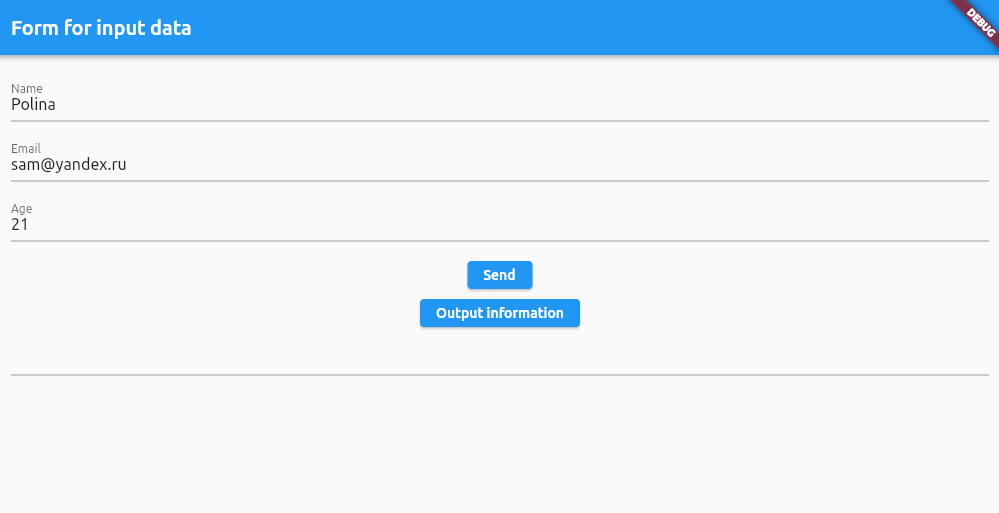
\includegraphics[width=0.8\textwidth]{img1}
\caption{Ввод данных}
\label{fig:img1}
\end{figure}

\begin{figure}[!htb]
	\centering
	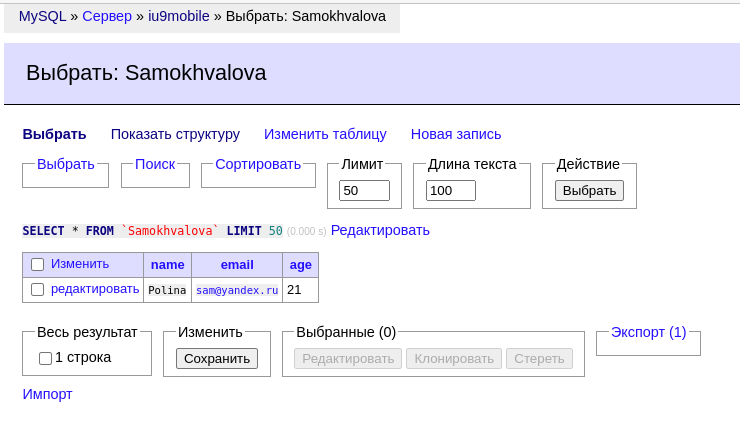
\includegraphics[width=0.8\textwidth]{img2}
\caption{Данные в таблице}
\label{fig:img2}
\end{figure}

\begin{figure}[!htb]
	\centering
	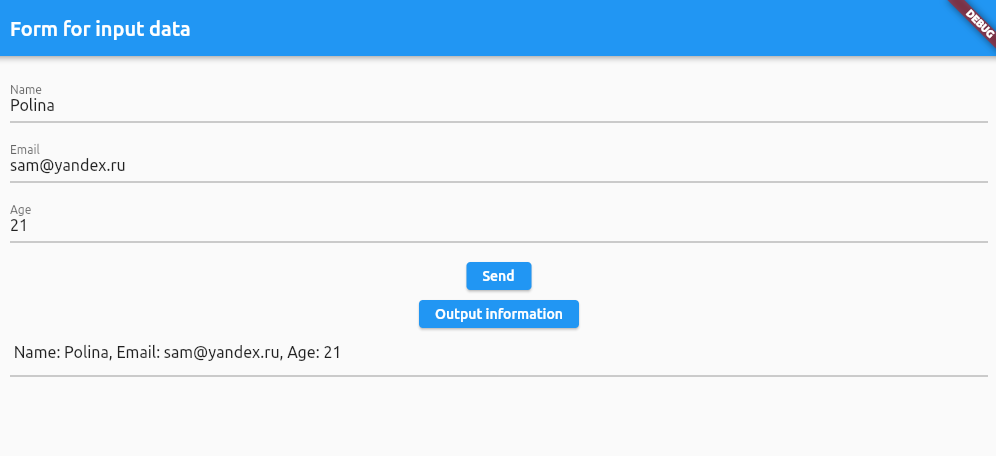
\includegraphics[width=0.8\textwidth]{img3}
\caption{Получение данных из базы данных}
\label{fig:img3}
\end{figure}

\section{Выводы}\label{Sect::conclusion}

В результате выполнения летучки была реализована форма отправки имени, адреса электронной почты и возраста пользователя в базу данных MySQL, было реализовано отображение текущего содержимого таблицы.
\end{document}
